\section{Plant nutrition}
\subsection{Photosynthesis}

As discussed before, all organisms derive their energy through respiration of glucose, but they
must get the glucose from somewhere. Most animals eat plants for their glucose, plants make their
own glucose by photosynthesis.

In photosynthesis, using energy from the sun trapped by chlorophyll, carbon dioxide and water are
synthesised into glucose and oxygen, a fact that can be shown in the following word and chemical
symbol equations:
\begin{center}
	\ce{carbon dioxide + water ->[$\Pi$] glucose + oxygen}

	\ce{ 6CO2 + 6H2O ->[$\Pi$] C6H12O6 + 6O2}
\end{center}
where $\Pi$ represents energy from sunlight trapped by chlorophyll.

Note that it is chlorophyll that is responsible for turning light energy to chemical energy 
required for photosynthesis.

This formed glucose can be used directly for respiration in the plant. However, when energy is not
immediately needed, it can be converted to starch to be used as an energy store. It may be 
converted to cellulose to make the plant's cell walls. To be transported through the plant, starch
is converted to sucrose before being converted to glucose.

A variegated leaf is that which lacks chlorophyll and hence green colour in some places. When we
test for starch using iodine in these places which lack chlorophyll, the result is negative, which
shows that chlorophyll is definitely required for photosynthesis.

When a leaf is covered with black paper and kept in a place with plenty of light, after starch
test it is observed that only the places that were uncovered have starch, meaning the covered
part of the leaf did not perform photosynthesis due to lack of light.

Potassium hydroxide solution, KOH, absorbs carbon dioxide. When a leaf is kept in a closed 
container in presence of this solution, that closed container has all its carbon dioxide absorbed
by the potassium hydroxide. The leaf has no carbon dioxide near it. Starch test shows absence of
starch. This means carbon dioxide is required for photosynthesis.

\begin{center}
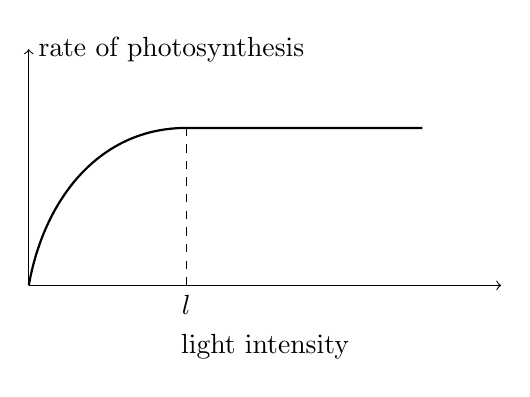
\begin{tikzpicture}
    % Axes
    \draw[->] (0,0) -- (6,0); % x-axis
	\draw[->] (0,0) -- (0,3) node[right] {rate of photosynthesis}; % y-axis

	\draw (3, -0.5) node[below] {light intensity};

    % Draw the curve: increasing, decreasing rate, and then flat
    \draw[thick] (0,0) to[out=80, in=180] (2,2) to[out=0, in=180] (5,2);

    % Label the levelling off point as 'l' below the x-axis
    \node at (2,0) [below] {$l$};

    % Add dashed line to show the transition to straight
    \draw[dashed] (2,0) -- (2,2);
\end{tikzpicture}
\end{center}
The above graph shows the rate of photosynthesis when plotted against light intensity. At low light,
there is no photosynthesis and it increases as light intensity increases. Beyond light intensity
$l$, rate of photosynthesis does not increase further. When light intensity is less than $l$, the
limiting factor is the light intensity, beyond it some other factor is limiting rate of photosynthesis.

The same pattern is seen for carbon dioxide concentration in the atmosphere:
\begin{center}
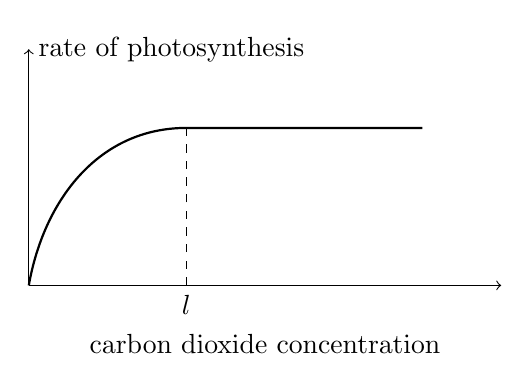
\begin{tikzpicture}
    % Axes
    \draw[->] (0,0) -- (6,0); % x-axis
	\draw[->] (0,0) -- (0,3) node[right] {rate of photosynthesis}; % y-axis

	\draw (3, -0.5) node[below] {carbon dioxide concentration};

    % Draw the curve: increasing, decreasing rate, and then flat
    \draw[thick] (0,0) to[out=80, in=180] (2,2) to[out=0, in=180] (5,2);

    % Label the levelling off point as 'l' below the x-axis
    \node at (2,0) [below] {$l$};

    % Add dashed line to show the transition to straight
    \draw[dashed] (2,0) -- (2,2);
\end{tikzpicture}
\end{center}

Temperature also affects rate of photosynthesis. This comes down to the fact that some of the
reactions involved in photosynthesis are enzyme controlled, and the curve when rate of photosynthesis
is plotted against temperature looks very similar to that when enzyme activity is plotted against
temperature. It shows that plants have an optimum temperature for maximum photosynthesis, $o$ in
the following graph:

\begin{center}
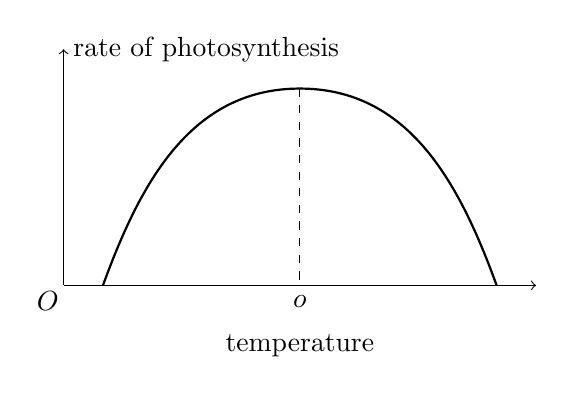
\begin{tikzpicture}

% Axes
\draw[->] (0,0) -- (6,0);
\draw (3, -0.5) node[below]{temperature};
\draw[->] (0,0) -- (0,3) node[right] {rate of photosynthesis};

% Enzyme activity curve (bell-shaped)
\draw[thick] (0.5,0) to[out=70, in=180] (3,2.5) to[out=0, in=110] (5.5,0);

% Dashes to x-axis (example points)
\draw[dashed] (3,2.5) -- (3,0) node[below] {$o$};

% Origin label
\node at (-0.2,-0.2) {$O$};

\end{tikzpicture}
\end{center}

Throughout this entire graph, temperature is indeed the limiting factor.

\subsection{Leaf structure}

Leafs are structures in plants which are the site of photosynthesis,
more specifically, chloroplasts in these leaves are the sites of photosynthesis. They are broad, 
to maximise
contact with sunlight to absorb energy. This broadness also maximises surface area to absorb
as much carbon dioxide as possible.
They are thin so that sunlight can pass right through them
and so that carbon dioxide diffuses quickly to all the cells.

The cross section of a leaf consists of many layers. First is the upper epidermis, where tightly
packet cells reduce the quantity of water vapour escaping from the leaf. These lack chloroplasts and
hence cannot photosynthesise. They produce a waxy, thin, transparent covering called the made of
a waxy substance. This layer is called the cuticle.

The subsequent layer is the palisade mesophyll, the first part of the mesophyll layer. These are
tall, regularly shaped narrow cells containing high numbers of chloroplasts. They get the maximum
exposure to sunlight and hence photosynthesise as the layer above them is transparent.

The layer below the palisade mesophyll is the spongy mesophyll, the last part of the mesophyll layer.
These contain not as many chloroplasts and are not as tightly packed as the palisade mesophyll cells.
The air spaces between these relatively irregularly shaped cells allow carbon dioxide and oxygen
to diffuse between the air and the cells inside the leaf and also allow water vapour to move from
the surface of the cells to outside the leaf.

Vascular bundles are also present in the spongy mesophyll, consisting of tubes called xylem and 
phloem, which are involved in the transport system of plants (see Section 7).

The last layer is called the lower epidermis, which, on some plants makes a cuticle and some it
does not as it is not often exposed to sunlight and hence not much water vapour can be lost from
this side. There are openings in this layer called stomata, which are surrounded by a pair of
guard cells. These guard cells change their shape, allowing diffusion of oxygen and carbon dioxide
in and out from the leaf by opening or closing the stomata. These guard cells also contain 
chloroplasts so as to make their own glucose for when they need to respire to open and close.

\subsection{Mineral nutrition}

For plants, absorption of nitrate ions from the soil is important for making amino acids, which is
required for the production of proteins. Magnesium ions are required to make chlorophyll, which
must also be absorbed from the soil.
